%% Be sure to check spelling!

%% Put your name and the proper due date in place

%% Copy the lstinputlisting and figure code as many times as you need; be sure to put in your own file names if appropriate

%% Note that the \includegraphics and \lstinputlisting commands are currently commented out with %%% - until the files exist, processing this code without them will result in an error so leave the comments until you have created the files!

\documentclass{article}
\usepackage{amsmath}    % loads AMS-Math package
\usepackage{graphicx}   % allows image files
\usepackage{listings}   % allows lstlisting environment
\usepackage[letterpaper, margin=0.75in]{geometry}  % set paper size/margins
\usepackage{EGR103style} % colorful file imports

\begin{document}
\begin{center}
\rule{6.5in}{0.5mm}\\~\\
\textbf{\large EGR 103L -- Spring 2021}\\~\\
\textbf{\huge Structured Programming I}\\~\\
***NAME (NetID)***\\
***Lab Section N, DAY TIMES***\\
***DATE DUE***\\~\\
{\small I understand and have adhered to all the tenets of the Duke
  Community Standard in completing every part of this assignment.  I
  understand that a violation of any part of the Standard on any part
  of this assignment can result in failure of this assignment, failure
  of this course, and/or suspension from Duke University.} 
\rule{6.5in}{0.5mm}\\
\end{center}
\tableofcontents
\listoffigures
\pagebreak

\section{Sinusoids}
%%% Discussion

\section{Chapra Problem 3.10}
%%% Replace the spaces (~) belowwith the appropriate numbers
\begin{itemize}
\item max\_pos\_disp = ~
\item max\_pos\_disp\_loc = ~ ft
\item max\_neg\_disp = ~
\item max\_neg\_disp\_loc = ~ ft
\end{itemize}

\pagebreak
\appendix
\section{Codes}
% Put the name of your file in the subsection name 
% and the lstinputlisting - note that _ need to be \_ in 
% subsection name but not in lstinpustlisting name!

% Be sure to include the community standard in codes!

% Add \pagebreaks if they make sense


% Set default to python
\lstset{style=python103, language=python} 

%%% Copy this as many times as needed for your files;
%%% Remove %%% from lstinputlisting when ready
%%% Note required \_ in subsection name versus _ in file name.

\subsection{FILE\_NAME.py}
%\lstinputlisting{FILE_NAME.py}

\clearpage % start Figures on new page

\section{Figures}
% Remove %%% when ready; use your file names if different from mine
\begin{figure}[ht!]
\begin{center}
%%%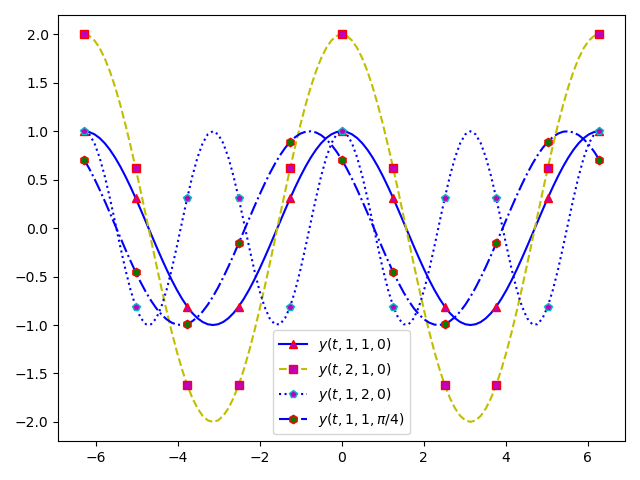
\includegraphics[width=5in]{cosine_plot.png}
\caption{Four sinusoids.}
\end{center}
\end{figure}

\begin{figure}[ht!]
\begin{center}
%%%\includegraphics[width=5in]{DisplacementPlot.eps}
\caption{Displacement plot for a beam.}
\end{center}
\end{figure}

\end{document}
